\documentclass[../differential_geometry.tex]{subfiles}
\begin{document}
\section{Aula 13 - de Fevereiro, 2026}
\subsection{Motivações}
\begin{itemize}
	\item Isometrias.
\end{itemize}
\subsection{Isometrias}
Seja S uma superfície regular em \(\mathbb{R}^{n}\) e considere a primeiro forma fundamental \(I_p:T_{p}S\rightarrow \mathbb{R}\) com
\[
	I_{p}(w) = \langle w, w \rangle_{p}.
\]
Se \(\underline{x}:U\rightarrow S\) é uma parametrização local de S, temos
\[
	I_{p}(a\underline{x}_u + b \underline{x}_v) = a^{2}E + 2ab F + b^{2}G,
\]
onde \(E,\; F, \; G\) são os coeficientes da primeira forma fundamental, como vimos previamente. A métrica associada à primeira forma é
\[
	\mathrm{d}s^{2} = E \mathrm{d}u^{2} + 2F \mathrm{d}u\mathrm{d}v + G^{2}\mathrm{d}v^{2}.
\]
\begin{def*}
	Dada uma métrica em S, o \textbf{comprimento de curvas em S} é calculado como
	\[
		\ell (\alpha ) = \int_{s_{0}}^{s}((u')^{2} + 2u'v'F + (v')^{2}G)^{\frac{1}{2}} \mathrm{d}t, \quad \alpha (t) = \underline{x}(u(t), v(t)). \; \square
	\]
\end{def*}
Seja \(f:S\rightarrow \tilde{S}\) uma aplicação suave entre as superfícies S e \(\tilde{S}\); se f preserva a métrica, ou seja, se
\[
	\langle w_1, w_2 \rangle_{p} = \langle \mathrm{d}f_{p}(w_1), \mathrm{d}f_{p}(w_2) \rangle_{f(p)},
\]
então fazer medidas em S torna-se equivalente a fazer medidas em \(\tilde{S}\)! É como se \(S\) e \(\tilde{S}\) fossem ``uma mesma superfície'', pelo menos em relação à métrica.
\begin{example}[Isometria Cilindro e Feixe do Plano]
	Pela função
	\[
		f(u, v) = (\cos^{}{u}, \sin^{}{u}, v), \quad 0\leq u\leq 2\pi ,\; v\in \mathbb{R},
	\]
	o cilindro é metricamente uma faixa de um plano:
	\begin{figure}[H]
		\begin{center}
			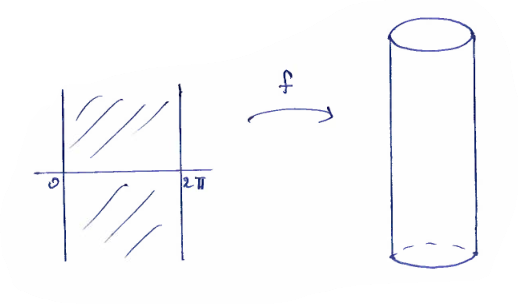
\includegraphics[height=0.8\textheight, width=0.8\textwidth, keepaspectratio]{./Images/cylinder_isometry_13.png}
		\end{center}
	\end{figure}
	Vamos parametrizar os dois para computar o comprimento de uma curva no cilindro. Para o plano, parametrizamos com \(E = 1, F = 0\) e \(G = 1\):
	\begin{align*}
		 & \underline{x}(u, v) = (u, v, 0) \\
		 & \underline{x}_{u} = (1, 0, 0)   \\
		 & \underline{x}_{v} = (0, 1, 0).
	\end{align*}
	No cilindro, de forma similar, colocamos
	\begin{align*}
		 & y(u, v) = (\cos^{}{u}, \sin^{}{u}, v)            \\
		 & \underline{y}_{u} = (-\sin^{}{u}, \cos^{}{u}, 0) \\
		 & \underline{y}_{v} = (0, 0, 1),
	\end{align*}
	dando também \(E =1, F=0\) e \(G=1\).

	Agora, seja \(\alpha (t) = (u(t), v(t), 0)\) uma curva no plano; temos
	\[
		\ell (\alpha ) = \int_{t_{0}}^{t}\sqrt[]{(u')^{2}+2u'v' \cdot 0 + (v')^{2}} \mathrm{d}s = \int_{t_{0}}^{t}\sqrt[]{(u')^{2} + (v')^{2}} \mathrm{d}s.
	\]
	No cilindro, a imagem de \(\alpha \) é
	\begin{align*}
		\beta (t) = f(\alpha (t)) & = (\cos^{}{u(t)}, \sin^{}{u(t)}, v(t)) \\
		                          & = \underline{y}(u(t), v(t)),
	\end{align*}
	e seu comprimento é
	\[
		\ell (f(\alpha )) = \int_{t_{0}}^{t}\sqrt[]{(u')^{2} + (v')^{2}} \mathrm{d}s = \ell (\alpha ).
	\]
\end{example}
\begin{def*}
	Uma aplicação \(f:S\rightarrow \tilde{S}\) entre duas superfícies suaves é uma \textbf{isometria local} se
	\[
		\langle \mathrm{d}f_{p}(w_1), \mathrm{d}f_{p}(w_2) \rangle_{f(p)} = \langle w_1, w_2 \rangle_{p},\quad \forall w_1, w_2\in T_{p}S,\; \forall p\in S.
	\]
	Neste caso, dizemos que S e \(\tilde{S}\) são \textbf{localmente isométricas}.

	Mais ainda, se f é um difeomorfismo, então dizemos que f é uma \textbf{isometria} e que S e \(\tilde{S}\) são \textbf{isométricas}. \(\square\)
\end{def*}
\begin{example}
	O cilindro e o plano são localmente isométricos, mas não são isométricos.
\end{example}

Observe que uma isometria local preserva as primeiras formas fundamentais, ou seja, preserva as métricas; além disso, se f é uma isometria local, então \(\mathrm{d}f_p:T_{p}S\rightarrow T_{f(p)}\tilde{S}\) é um isomorfismo: de fato,
\[
	\mathrm{d}f_p(w) = 0 \Longleftrightarrow \langle \mathrm{d}f_p(w), \mathrm{d}f_p(w) \rangle_{f(p)}=0 \Longleftrightarrow \langle w, w \rangle_p = 0 \Longleftrightarrow w = 0.
\]
\begin{prop*}
	Seja \(\underline{x}:U\rightarrow S\) uma parametrização local de S. A aplicação \(f:S\rightarrow \tilde{S}\) é uma isometria local em \(\underline{x}(U)\) se, e somente se,
	\[
		\langle f_u, f_u \rangle = E,\; \langle f_u, f_v \rangle = F,\; \langle f_v, f_v \rangle = G,
	\]
	onde E, F e G são os coeficientes da primeira forma fundamental de S com relação a \(\underline{x}\).
\end{prop*}
\begin{proof*}
	Suponha que f é uma isometria local:
	\[
		\langle \mathrm{d}f_p(w_1), \mathrm{d}f_p(w_2) \rangle_{f(p)} = \langle w_1, w_2 \rangle, \quad \forall w_1, w_2\in T_pS,\; p\in \underline{x}(U);
	\]
	então,
	\[
		\langle f_u, f_u \rangle = \langle \mathrm{d}f_p(\underline{x}_u), \mathrm{d}f_p(\underline{x}_u) \rangle = \langle \underline{x}_u, \underline{x}_u \rangle = E,
	\]
	e de forma análoga,
	\[
		\langle f_u, f_v \rangle = F \quad\&\quad \langle f_v, f_v \rangle = G.
	\]

	Para a recíproca, sejam \(w_1 = a \underline{x}_u + b\underline{x}_v,\; w_2 = c \underline{x}_u + d \underline{x}_v\) em \(T_pS\); basta notar a conta:
	\begin{align*}
		\langle \mathrm{d}f_p(w_1), \mathrm{d}f_p(w_2) \rangle & = \langle \mathrm{d}f_p(a\underline{x}_u + b\underline{x}_v), \mathrm{d}f_p(c\underline{x}_u + d \underline{x}_v) \rangle                                                   \\
		                                                       & = ac \langle \mathrm{d}f_p(\underline{x}_u), \mathrm{d}f_p(\underline{x}_u) \rangle + (ad+bc)\langle \mathrm{d}f_p(\underline{x}_u), \mathrm{d}f_p(\underline{x}_v) \rangle \\
		                                                       & \quad +bd \langle \mathrm{d}f_p(\underline{x}_v), \mathrm{d}f_p(\underline{x}_v) \rangle                                                                                    \\
		                                                       & = ac \langle f_u, f_u \rangle + (ad+bc)\langle f_u, f_v \rangle + bd \langle f_v, f_v \rangle                                                                               \\
		                                                       & = acE + (ad+bc)F + bd G                                                                                                                                                     \\
		                                                       & = \langle w_1, w_2 \rangle. \text{ \qedsymbol}
	\end{align*}
\end{proof*}
Há um caso particular, ilustrado na proposição seguinte:
\begin{prop*}
	Suponha que \(\underline{x}:U\rightarrow S\), que \(\underline{\tilde{x}}:U\rightarrow \tilde{S}\) são parametrizações locais de S e \(\tilde{S}\), e que \(E,\; F,\; G,\; \tilde{E},\; \tilde{F},\; \tilde{G}\) são os coeficientes de suas respectivas primeiras formas fundamentais. Então,
	\[
		f:\underline{\tilde{x}}\circ \underline{x}^{-1}: \underline{x}(U)\rightarrow \underline{\tilde{x}}(U)
	\]
	é uma isometria local se, e somente se,
	\[
		E = \tilde{E}, \quad F = \tilde{F}, \quad G = \tilde{G}.
	\]
	\begin{figure}[H]
		\begin{center}
			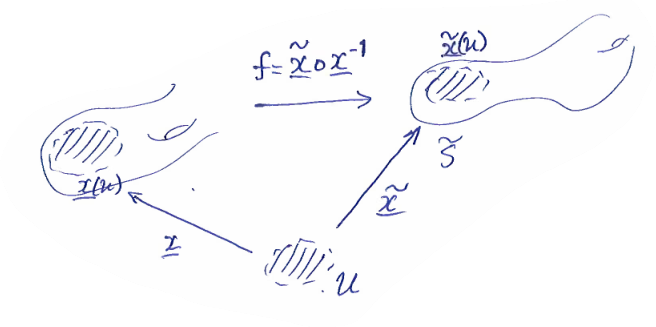
\includegraphics[height=\textheight, width=\textwidth, keepaspectratio]{./Images/proposition_13.png}
		\end{center}
	\end{figure}
\end{prop*}
\begin{proof*}
	Pela proposição anterior, f é uma isometria local se, e somente se,
	\[
		E = \langle f_u, f_u \rangle = \langle (f\circ \underline{x})_{u}, (f\circ \underline{x})_{v} \rangle = \langle \underline{\tilde{x}}_{u}, \underline{\tilde{x}}_{u} \rangle = \tilde{E},
	\]
	e similarmente para F e G.

	Como exercício, prove que f é um difeomorfismo. \qedsymbol
\end{proof*}
\begin{exr}
	Finalize a prova acima.
\end{exr}
\begin{example}[Retomando Cilindro e Feixe]
	No mesmo contexto do caso anterior, temos os coeficientes
	\[
		E = \tilde{E} = 1,\quad F = \tilde{F} = 0 \quad\&\quad G = \tilde{G} = 1.
	\]
	\begin{figure}[H]
		\begin{center}
			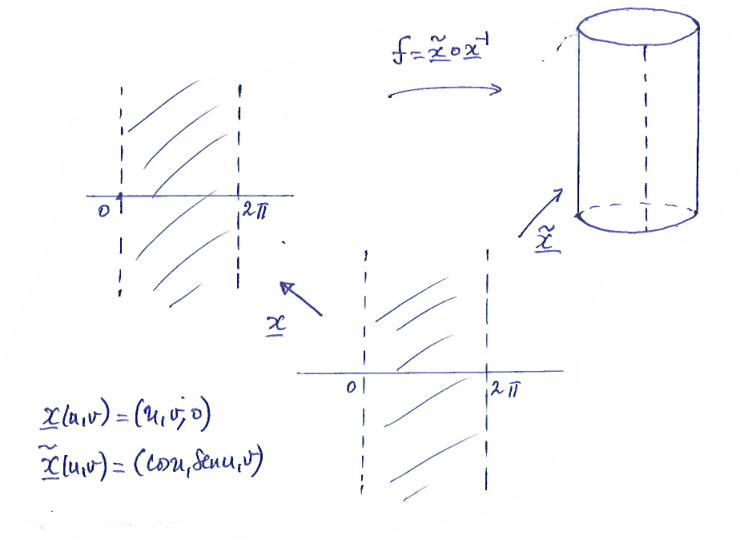
\includegraphics[height=\textheight, width=\textwidth, keepaspectratio]{./Images/plane_isometry_13.png}
		\end{center}
	\end{figure}
	Portanto, \(f = \underline{\tilde{x}}\circ \underline{x}^{-1}\) é uma isometria da faixa do plano \(0 < x < 2\pi ,\; y\in \mathbb{R},\; z=0\) ao cilindro, a menos de uma reta.
\end{example}

\begin{example}[Catenoide e Helicoide]
	A catenoide é parametrizada por
	\[
		\underline{x}(u, v) = (\cosh^{}{v}\cos^{}{u}, \cosh^{}{v}\sin^{}{u}, v), \quad (u, v)\in (0, 2\pi )\times \mathbb{R} = U,
	\]
	tal que
	\[
		E = \cosh^{2}{v},\quad  F = 0 \quad\&\quad G = \cosh^{2}{v}.
	\]

	A helicoide, por outro lado, é
	\[
		\underline{\tilde{x}}(u, v) = (\sinh^{}{v}\cos^{}{u}, \sinh^{}{v}\sin^{}{u}, u), \quad (u, v)\in (0, 2\pi )\times \mathbb{R} = U.
	\]
	Neste caso,
	\[
		\tilde{E}=\cosh^{2}{v},\quad \tilde{F} = 0 \quad\&\quad \tilde{G} = \sinh^{2}{v}.
	\]
	Logo, \(f=\tilde{x}\circ x^{-1}\) é uma isometria entre \(\underline{x}(U)\) e \(\tilde{x}(U)\).
\end{example}
\begin{exr}
	Mostre que um difeomorfismo \(f:S\rightarrow \tilde{S}\) é uma isometria se, e somente se, o comprimento do arco de qualquer curva parametrizada em S é igual ao comprimento da sua imagem em \(\tilde{S}\) por f.
\end{exr}
\begin{exr}
	Existe uma isometria local entre um plano e a esfera?
\end{exr}
\end{document}

